\documentclass[orivec]{llncs}
\usepackage{graphicx}
\usepackage{amsmath}			% for "cases"
\usepackage{amsfonts}		% for frakur fonts
\usepackage{mathrsfs}		% for curly "E" error symbol
\usepackage{float}
\usepackage[most]{tcolorbox}	% for wrapping example in color box
% \usepackage{wrapfig}			% wrap figure beside text, used in example
\usepackage{tikz-cd}			% commutative diagrams
\usepackage{tikz}
\usepackage{amssymb}			% for \multimap \updownarrow \bigstar \varnothing
\usepackage{sectsty}			% change section color
% \usepackage{turnstile}		% longer turnstiles
\usepackage{wasysym}			% smileys
\usepackage[normalem]{ulem}	% underline with line breaks: /uline
\usepackage{hyperref}		% refs, links become clickable
\usepackage[]{algorithm2e}	% algorithms

\usepackage{geometry}		% change paper size
\geometry{
  a4paper,         % or letterpaper
  textwidth=18cm,  % llncs has 12.2cm
  textheight=27cm, % llncs has 19.3cm
  heightrounded,   % integer number of lines
  hratio=1:1,      % horizontally centered
  vratio=2:3,      % not vertically centered
}
\usepackage[fontsize=13pt]{scrextend}

% *************** Delete when not using Chinese or colors **********************
\usepackage{xeCJK}
\setCJKmainfont[BoldFont=SimHei,ItalicFont=KaiTi]{SimSun}
\usepackage{color}
\definecolor{cerulean}{RGB}{100,100,200}
%\newcommand{\emp}[1]{\textbf{\textcolor{Cerulean}{#1}}}
\newcommand{\emp}[1]{\textbf{#1}}
\definecolor{grey}{rgb}{0.9,0.9,0.9}  % grey

% \chapterfont{\color{blue}}  % sets colour of chapters
\sectionfont{\color{blue}} 
\subsectionfont{\color{blue}} 
\subsubsectionfont{\color{blue}} 
\setcounter{secnumdepth}{3}		% use numbers in subsubsections

\let\emptyset\varnothing			% more beautiful empty set symbol
\newcommand{\vect}[1]{\boldsymbol{#1}}
\newcommand*\sigmoid{\vcenter{\hbox{
\includegraphics{sigmoid.png}}}}
\newcommand*\KB{\vcenter{\hbox{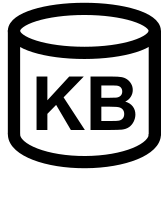
\includegraphics{KB-symbol.png}}}}
\newcommand*\NN{\vcenter{\hbox{\includegraphics{NN-symbol.png}}}}
\newcommand*\invsigmoid{\vcenter{\hbox{\includegraphics{inverse-sigmoid.png}}}}
\newcommand{\invW}{\, \rotatebox[origin=c]{90}{W}}
\newcommand{\invw}{\, \rotatebox[origin=c]{90}{w}}
\newcommand*\rectifier{\vcenter{\hbox{\includegraphics{rectifier.png}}}}
\newcommand{\dashh}{\textemdash~}

\newcommand{\tikzmark}[1]{\tikz[overlay,remember picture] \node (#1) {};}

\renewcommand{\thefootnote}{\fnsymbol{footnote}}
\interfootnotelinepenalty=10000

% ***** Boxed variables inside math equations
% \newcommand*{\boxedcolor}{black}
\makeatletter
% \renewcommand{\boxed}[1]{\textcolor{\boxedcolor}{%
% \fbox{\normalcolor\m@th$\displaystyle#1$}}}
% \setlength{\fboxsep}{1pt}
\renewcommand{\boxed}[1]{\fbox{\m@th$\displaystyle\scalebox{0.9}{#1}$} \,}
\makeatother

\overfullrule=0mm

\newsavebox{\MyName}
\savebox{\MyName}{
\includegraphics[scale=0.6]{YKY.png}}

\title{什么是 kNN 算法?(What is k-nearest-neighbor?)}
\titlerunning{什么是 kNN 算法?}
\author{\usebox{\MyName} (King-Yin Yan)
% \\ \footnotesize{General.Intelligence@Gmail.com}
}
\institute{General.Intelligence@Gmail.com}

\begin{document}

\maketitle
\setlength{\parindent}{0em}
% \setlength{\parskip}{2.8ex plus0.8ex minus0.8ex}
\setlength{\parskip}{2.8ex}

%\begin{abstract}
%\end{abstract}

学习 machine learning 的最低要求是什么?  我发觉要求可以很低,甚至初中程度已经可以。  首先要学习一点 Python 编程,譬如这两本小孩子用的书:\href{http://www.manning.com/sande/}{【1】} \href{http://item.jd.com/11410467.html}{【2】} 便可。  数学方面,只需要知道「两点间距离」的公式(中学的座标几何会读到)。

这本书第二章介绍 kNN 算法,包括 Python 程序:
\begin{equation}
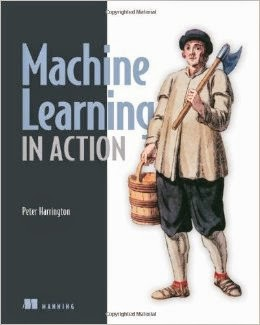
\includegraphics[scale=0.75]{machine-learning-in-action(cover).jpg}
\end{equation}

其他章节的数学要求可能不同,但我目的是想说明,很多实用的人工智能的原理,其实也很简单的。

kNN 是什么?  For example:
\begin{equation}
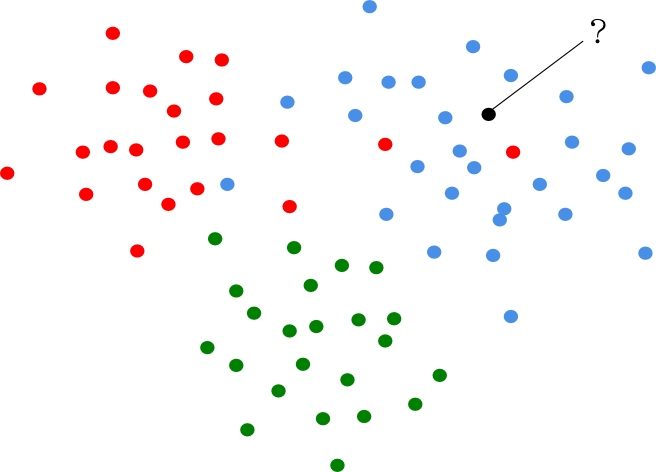
\includegraphics[scale=0.6]{kNN-example.png}
\end{equation}

开始时,所有 data points 的 labels (颜色)已经是知道的。

kNN 要解决的问题是:  图中那「?」点的 label 应该是什么颜色?

用肉眼直观来看,那「?」的位置,是在{\color{cerulean}蓝色}点密集的区域,所以最「贴切」的标签应该是{\color{cerulean}蓝色}。

kNN 的算法就是:
\let\labelitemi\labelitemii
\begin{itemize}
\item 在已知的 data points 中,逐一点检视(把這每一點叫作 P):
\begin{itemize}
\item 首先计算「?」和 P 之间的距离
\end{itemize}
\item 所有距离计算之后,将他们由小至大 sort 好
\item 从 sort 好的序列,取最前的 k 个(即距离最接近「?」的 k 个点子)
\item 对这 k 个点,读出他们的 label(颜色)是什么,这是问题中已经知道的
\item 所有这些 labels(颜色),哪个出现最多?  (亦即是说,最接近「?」的 k 个点子,它们最普遍是什么颜色?)
\item 这出现次数最多的颜色,就是答案
\end{itemize}

例如,使用者要求 k = 5 时:
\begin{equation}
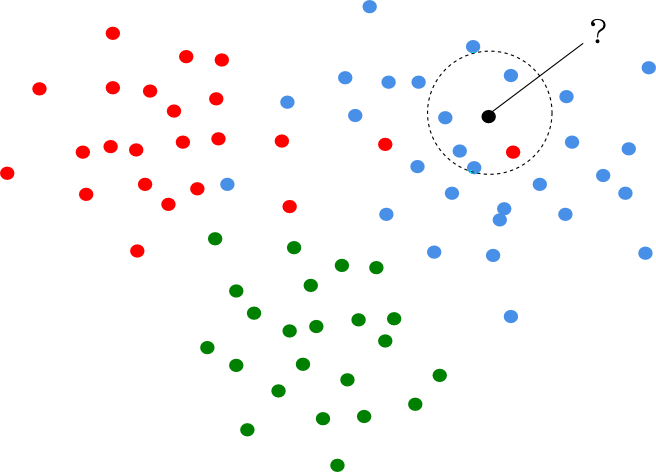
\includegraphics[scale=0.6]{kNN-example2.png}
\end{equation}

\newcommand{\balla}{{\color{cyan} \Large $\bullet$}}
\newcommand{\ballb}{{\color{red} \Large $\bullet$}}
最接近「?」的 5 个点,就是以「?」为中心的虚线圆圈内的 5 个点。  它们的颜色顺序依次为:[\balla ,\ballb,\balla,\balla,\balla ] 。 出现的次数是 4\balla ~ 1\ballb ,所以最高次数的颜色是 \balla 。

\section{如何用 Python 写 kNN ?}

\subsection{计算点与「?」之间距离}

首先,回忆中学的坐标几何里,两点间距离的公式。  假设那两点是 A 和 B,它们的座标分别是 $(x_A, y_A)$ 和 $(x_B, y_B)$,则:
\begin{equation}
\mbox{distance D} = \sqrt{ (x_A - x_B)^2 + (y_A - y_B)^2 }
\end{equation}
注意,在这公式里,用 $x_A - x_B$ 还是 $x_B - x_A$ 是没有分别的,因为那是正数和负数的分别,而在 $()^2$ 之后便没有分别。(换句话说,计算 A,B 之间的距离,和计算 B,A 之间的距离,是一样的。)

每个点子有 3 个坐标,分别是: x = 「坐飞机旅程」、y = 「吃雪糕的量」、z = 「玩电玩时间」,而 labels 是: 「很喜欢」、「普通喜欢」、「不喜欢」。

因为坐标有 3 个,所以处理的空间是 3 度空间,但为了初学者方便,我们只考虑其中两个座标,所以局限在 2 度空间(平面上)。   如果要 generalize 到 N-度空间,那需要用到 N-度空间中 两点间距离的公式,留给读者作为练习 {\Large \smiley}

写程式时,首先要知道那些点子是如何储存於某个 variable 中。  在书中的 ``dating'' 例子里,那些点子的坐标是 datingDataMat,而 labels 是储存在 datingLabels。

(妳可以在 Python 命令行,呼叫 file2matrix 函数去准备那些点子,然后试试印出 datingDataMat 和 datingLabel 这两个 variables 的内容。 例如 datingDataMat[ : , 1 ] 可以印出所有点子的第二个坐标(即吃雪糕量)。 那「:」的意思是,不指定指标的 begin 和 end,所以是对那个指标「全取」。)

我们用比较浅显的方法重写书中的 Python 函数(書裡的程式用了 vector 和 matrix 的表示法,比較簡潔,但較難懂):
\begin{verbatim}
    def classify1(inP, dataSet, labels, k):
        N = len(dataSet)
        Ds = array([0] * N)
        for i in range(N):
             x2 = (inP[0] - dataSet[i][0])**2
             y2 = (inP[1] - dataSet[i][1])**2
             D = sqrt(x2 + y2)
             Ds[i] = D
\end{verbatim}

第 1 句: 定义我们的 function。  inP 是 input point 的意思。

第 2 句: N 是我们 dataSet 的 size,即总共有多少点子。

第 3 句: 我们要计算距离 D,而且有 N 个这样的距离,所以要将结果储存在 array 里。  但使用 array 之前,要先定义它,并填上 0(这叫初始化,initialize)。  Ds 这名字的意思是「多个D」(如英语中的 dogs = dog 的众数)。

第 4 句是 loop:  对於每一点,我们用 i 这个 index「指着」它。  Index 是处理 array 的惯用做法,因为 array 容许妳读取任意位置的元素。

第 5、6 句:  计算 $\Delta x^2$ 和 $\Delta y^2$ 的值,注意,因为我们储存 x, y 的方法是 [x, y] 这样的 list, 所以 x 用指标 [0] 读取,y 用指标 [1] 读取。

第 7 句: 计算 $D = \sqrt{ \Delta x^2 + \Delta y^2 }$。

第 8 句: 将计算好的 D 放进 array Ds 里。

\subsection{将距离排序}

很简单,一句:
\begin{verbatim}
    Dsorted = Ds.sort()
\end{verbatim}
注意,這些程式段落要適當地 indent 好,不然 Python 會出錯的。  这句仍屬於 classify1 函数。

\subsection{读出点的颜色}

刚才说错了,因为 Ds 排序之后,再弄不清哪个点子对应於哪个 label,所以我们要用的是 ``arg sort'' (argument sort,即是用 \textbf{指标} 来排序)。

例如,设 a = array( [17, 38, 10, 49] ),\\
a.sort() 会给出 [10, 17, 38, 49],\\
但 a.argsort() 会给出 [2, 0, 1, 3],这些是 indices(指标)。\\
换句话说: argsort 的结果是 {\color{red} 旧的 indices 的新的排法}。

\begin{equation}
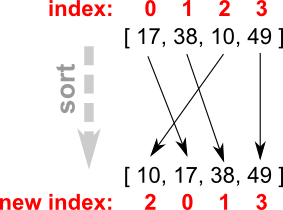
\includegraphics[scale=0.8]{arg-sort-explained.png}
\end{equation}

Python 程式:
\begin{verbatim}
    D_sorted = Ds.argsort()
    first_k = D_sorted[0:k]        # 提取前 k 个元素(但這句其實不需用到)
\end{verbatim}

现在要找出这 k 个点子的 labels,我们可以创造一个新的 array 储存它们:
\begin{verbatim}
    first_k_labels = array([0]*k)  # 准备空的 array
    for i in range(0,k):
        first_k_labels[i] = labels[ D_sorted[ i ]]
\end{verbatim}

最后那句要说明一下: 如果写 labels[i] 那就是第 i 个元素的 label。 但我们要的是 排序 好之后的元素的 label,所以我们先「look up」这个 D\_sorted array,找出排序后的元素的指标,再用那指标「look up」那 labels array。  (就像查字典,我们想查某个中文字的日语翻译,但我们只有汉英字典和英日字典,所以要两次 look up,出现了 array1[ array2[ i ] ] 这样的语法。 这是很常见的。)

\subsection{哪个颜色出现最多?}

用这个 loop 计算每个 label 出现的次数:
\begin{verbatim}
    like1 = 0              # 标签是「不喜欢这男孩」 的点的个数
    like2 = 0              # 标签是「普通喜欢这男孩」的点的个数
    like3 = 0              # 标签是「非常喜欢这男孩」的点的个数
    for i in range(0, k):
        label = first_k_labels[i]
        if label == 1:
            like1 += 1
        elif label == 2:
            like2 += 1
        elif label == 3:
            like3 += 1
\end{verbatim}

然后,找出出现次数最多那个 label:
\begin{verbatim}
    if like1 > like2 and like1 > like3:      # 如果 like1 出现最多
        best_label = 1                        # 答案是「不喜欢这男孩」
    elif like2 > like1 and like2 > like3:    # 如果 like2 出现最多
        best_label = 2                        # 答案是「普通喜欢这男孩」
    else:                                    # 如果 like3 出现最多
        best_label = 3                        # 答案是「非常喜欢这男孩」
\end{verbatim}

\subsection{完工!}

\begin{verbatim}
    return best_label
\end{verbatim}

\section{Testing}

实际的 Python program,还要加上这几行 ``header'':
\begin{verbatim}
# -*- coding: utf-8 -*-          # 加了這句可以用中文 comments

from numpy import array
from math import sqrt
\end{verbatim}

运行结果:
\begin{equation}
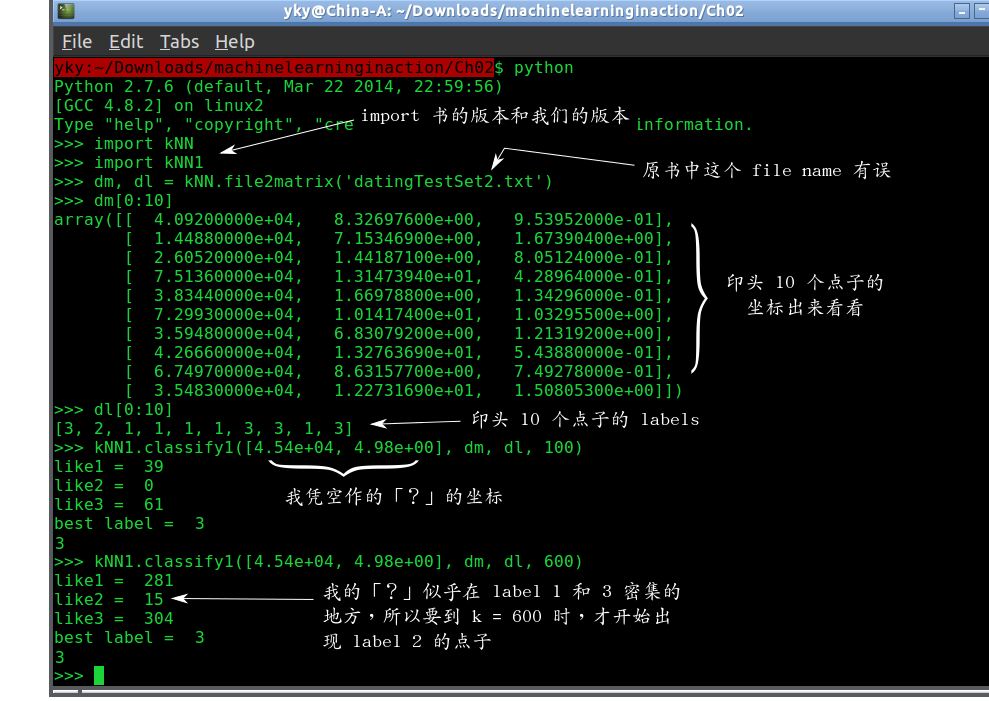
\includegraphics[scale=0.6]{execution.png}
\end{equation}

这例子里,「?」的坐标是 [4.54e+04, 4.98e+00],那是我看了数据后作出来的。 4.54e+04 是 scientific notation,即是 $4.54 \times 10^4$。

我把 k 增加到 600,才开始看到 like2 不是 0。

\quad \quad \quad --- 完 ---

\bibliographystyle{plain} % or number or aaai ...
\bibliography{AGI-book}

\end{document}
